\section{Discussion}\label{sec: discussion}

The results presented in the previous section show that exposure to the centralized school choice system leads to meaningful increases in  applications, assignments, and enrollment. In this section, we explore potential mechanisms that may help explain these patterns. 
To organize the discussion, we follow the framework in~\cite{larroucau2024}, where a student's optimal application list depends on three primitives: preferences over programs, beliefs about admission probabilities, and strategic behavior. Centralized school choice can affect college applications and outcomes through each of these channels. 
First, it may shift students' preferences over degree programs, for instance through peer effects: changes in the academic composition of schools may reshape aspirations, information about college options, or beliefs about expected returns to different programs.
Second, it may alter students' beliefs about admission probabilities—either because their actual application scores change (shifting true admission chances) or because exposure to a centralized system reduces biases in perceived admission chances (e.g., over- or under-confidence). 
Third, exposure to a centralized school‑choice system may alter students’ strategic behavior in later centralized admissions, giving them practical experience that improves application choices and reduces incentives to misreport preferences. We now discuss each of these mechanisms in more details.\footnote{This discussion is not intended to provide an exhaustive account of all possible drivers of the observed effects. Other channels—such as changes in students' awareness of available programs or their knowledge of program characteristics—may also play a role but are beyond the scope of our empirical tests. Our goal is to offer suggestive evidence on mechanisms that are plausibly at play and consistent with the institutional features of the reform. } 

% We focus on two channels that are especially salient in this context: (i) increased familiarity with centralized application and assignment processes, and (ii) peer effects operating through changes in school composition induced by the reform. This discussion is not intended to provide an exhaustive account of all possible drivers of the observed effects; rather, it aims to offer suggestive evidence on two mechanisms that are plausibly at play and consistent with the institutional features of the reform.





\subsection{Effect through Changes in Preferences}
Participation in a centralized, deferred-acceptance-based school-choice system can reshape students' preferences when they later apply to college through several channels. By coordinating applications and reallocating seats via priorities and lotteries, centralization alters both the perceived and realized probability of attending higher-quality secondary schools. For some students, this raises awareness and the expected returns to more ambitious college pathways and makes selective options appear attainable. In addition, exposure to higher-quality peers and teachers can increase aspirations, transmit application know-how, and foster norms around effort and postsecondary investment.

A key way to summarize these mechanisms is through changes in the degree and nature of segregation in the secondary system. \citet{urzua2023} show that Chile's centralized school choice reform did not generate meaningful changes in the socioeconomic composition of schools, with effects concentrated in areas characterized by high residential segregation or a strong private-school sector. However, their analysis focuses on socioeconomic segregation and does not examine the \emph{academic} composition of schools. This distinction is central in our context: a less segregated distribution of student ability implies that high-achieving students are more evenly spread across schools, increasing the likelihood that any given student is exposed to strong peers, higher expectations, and information about selective college options.
A large literature on peer effects shows that exposure to higher-achieving classmates can shape academic outcomes and educational trajectories through channels such as information transmission, encouragement, and the formation of norms around effort and postsecondary investment~\citep{hoxby2000b, Sacerdote2001, CarrellSacerdoteWest2013}. Thus, improvements in academic peer quality can plausibly increase students’ propensity to apply to, gain admission to, and ultimately enroll in college.\footnote{In Appendix~\ref{app: additional results} we examine whether participation in the centralized school-choice system affected the different types of admission-probability errors identified by \cite{larroucau2024}; we find no statistically significant effects. }

To examine whether the introduction of the centralized school choice system altered the \emph{academic} composition of schools, we study changes in segregation by ability using students' fourth-grade SIMCE scores in Math and Verbal as a measure of prior academic achievement. We construct three standard segregation indices at the district level: the Duncan index, which captures the unevenness in the distribution of low- and high-achieving students (relative to their district-year median) across schools; the exposure index ($P_{LH}$), which measures the average share of high-achieving peers faced by low-achieving students; and the isolation index ($P_{LL}$), which captures the extent to which low-achieving students are concentrated in schools with other low-achieving peers. Higher exposure and lower isolation indicate greater academic integration. Formal definitions and computational details for these indices are provided in Appendix~\ref{app: segregation measures}. We then estimate the effect of the reform on each segregation measure using a staggered Difference-in-Differences design at the district level, exploiting the sequential rollout of the centralized system across regions.

Table~\ref{tab: did segregation} reports the estimated average treatment effects. We find that joining the centralized school choice system leads to a negative and statistically significant effect on the Duncan index for both Math and Verbal SIMCE scores, indicating a reduction in segregation by academic ability. Consistent with this pattern, all coefficients are positive for $P_{LH}$ and negative for $P_{LL}$, i.e., the treatment increases the exposure of low-achieving students to high-achieving peers and decreases their isolation.
Taken together, these results point to a systematic decline in segregation by academic ability following the reform. 
% Such improvements in academic integration are consistent with the peer-effects mechanism discussed above: greater exposure to higher-achieving classmates may have contributed to the increases in college applications, admissions, and enrollment documented earlier.

\begin{table}[htbp]
   \caption{Effect on Segregation by Ability}\label{tab: did segregation}
   \centerline{\scalebox{0.85}{
\begin{tabular}{lcccccc}
\toprule
      & \multicolumn{2}{c}{Duncan Index} & \multicolumn{2}{c}{Exposure Low-High ($P_{LH}$)} & \multicolumn{2}{c}{Isolation Low-Low ($P_{LL}$)} \\
      \cmidrule(lr){2-3} \cmidrule(lr){4-5} \cmidrule(lr){6-7}
                   & Math & Verbal & Math & Verbal & Math & Verbal\\
                   & (1) & (2) & (3) & (4) & (5) & (6)\\
      \midrule
      Treated      & -0.035$^{***}$ & -0.024$^{***}$ & 0.053$^{***}$ & 0.042$^{***}$ & -0.053$^{***}$ & -0.042$^{***}$\\
                   & (0.008) & (0.009) & (0.008) & (0.010) & (0.008) & (0.010)\\
      \midrule
      Mean pre-treatment & 0.197 & 0.183 & 0.452 & 0.461 & 0.548 & 0.539\\
      Observations & 3,405 & 3,405 & 3,405 & 3,405 & 3,405 & 3,405 \\
      \bottomrule
\end{tabular}

}}
\end{table}


\subsection{Effect through Changes in Admission Probabilities and Beliefs}
Exposure to a centralized school-choice system may shape both students’ feasible choice sets and their beliefs about admission prospects when they later apply to college. On the one hand, centralized assignment can improve the match between students and secondary schools, allowing some students to attend higher-quality or better-fitting institutions. These improvements can translate into gains in academic achievement and preparation, thereby expanding the set of college options for which students are academically competitive and shifting revealed preferences toward more selective programs. On the other hand, participation in a centralized allocation mechanism may directly affect students' beliefs about admission probabilities. Through exposure to peers, school environments, and guidance from teachers, students may update their expectations about the likelihood of admission to different programs. In addition, the experience of participating in a system that explicitly links choices to probabilistic outcomes—through priorities,  and lotteries—may make the role of admission probabilities more salient, encouraging students to seek out and incorporate such information when forming their college application strategies.

We next examine the empirical relevance of these mechanisms. On the one hand, the results in Table~\ref{tab: main results} show no detectable effects on GPA or on the average score between the Math and Verbal components of the college entrance exam, suggesting that the mechanism operating through improvements in academic achievement and preparation is unlikely to be at play. Consistent with this interpretation, Table~\ref{tab: results by program selectivity} indicates that the observed gains in admissions are concentrated in less selective programs, providing no evidence of a shift toward more selective options.
On the other hand, Table~\ref{tab: effect on truthful reporting} shows that participation in the centralized school-choice system has no significant effect on students’ admission probabilities or on their biases when reporting their top choice or overall application. Overall, these results suggest that the policy does not meaningfully affect either students’ feasible sets—through academic preparation—or their beliefs about admission chances.

\begin{table}[!htbp]
\caption{Effect on Truthful Reporting}\label{tab: effect on truthful reporting}
\centerline{\scalebox{0.85}{
\begin{tabular}{lcccccc}
\toprule
 & \multicolumn{2}{c}{Truthful Reporting} & \multicolumn{2}{c}{Adm. Probability} & \multicolumn{2}{c}{Bias} \\
 \cmidrule(lr){2-3} \cmidrule(lr){4-5} \cmidrule(lr){6-7}
 & Top & Bottom & Top Reported & Overall & Top Reported & Overall \\
 & (1) & (2) & (3) & (4) & (5) & (6)\\
\midrule
 Treated & 0.093$^{***}$ & -0.001 & -0.023 & 0.005 & 0.021 & 0.017 \\
 & (0.028) & (0.001) & (0.030) & (0.016) & (0.025) & (0.015) \\
 Constant & 0.659$^{***}$ & 0.001 & 0.323$^{***}$ & 0.373$^{***}$ & 0.293$^{***}$ & 0.156$^{***}$ \\
 & (0.059) & (0.001) & (0.047) & (0.038) & (0.046) & (0.041) \\
\midrule
 Observations & 7,168 & 2,019 & 7,241 & 7,241 & 7,241 & 7,241 \\
\bottomrule
\end{tabular}
}}
\end{table}


\subsection{Effect through Changes in Application Behavior}

Participation in a centralized school-choice system also provides students with hands-on experience navigating a large, rule-based matching process, including submitting ranked preference lists, complying with deadlines, and interpreting assignment outcomes generated by a deferred-acceptance algorithm. This experience and the acquired procedural knowledge can reduce the cognitive and psychological costs of engaging with a similar system at the college level, particularly for students who might otherwise perceive the application process as complex or opaque. Furthermore, it may increase confidence in the system itself—both in its fairness and in the absence of costs or penalties from unsuccessful applications—thereby encouraging students to apply in the first place.

Beyond increasing participation, exposure to centralized assignment may also improve the quality of students' applications. First, familiarity with preference-based mechanisms may encourage students to submit longer and more complete application lists, as they better understand that applying to additional programs is typically costless and does not reduce admission chances at more preferred options. Second, procedural learning may reduce avoidable mistakes, such as applying to programs for which minimum requirements are not met, by improving students' ability to interpret eligibility criteria and admission thresholds. Finally, experience with a strategy-proof mechanism may promote more accurate preference revelation, as students learn that truthful reporting is optimal and need not be distorted by strategic concerns. Taken together, these channels suggest that centralized school choice can improve both the likelihood of applying and the quality of application decisions.

\begin{table}[htbp]
   \caption{Effect on College Application Quality}\label{tab: application quality}
   \centerline{\scalebox{0.85}{
\begin{tabular}{lccccc}
\toprule
      & \multicolumn{3}{c}{Application Breadth} & \multicolumn{2}{c}{Application Quality} \\
      \cmidrule(lr){2-4}\cmidrule(lr){5-6}
      & $\geq 1$ & $\geq 3$ & $\geq 5$ & Valid Apps & Above Cutoff \\
      & (1) & (2) & (3) & (4) & (5) \\
\midrule
      Treated & 0.054$^{***}$ & 0.031$^{***}$ & -0.075$^{***}$ & 0.134$^{***}$ & 0.034\\
       & (0.010) & (0.011) & (0.012) & (0.012) & (0.021)\\
      \midrule
      Mean (pre-treatment) & 0.426 & 0.362 & 0.226 & 0.725 & 0.480\\
      Observations & 28,483 & 28,483 & 28,483 & 27,491 & 27,491\\
\bottomrule
\end{tabular}
   }}
\end{table}


\marar{Table~\ref{tab: application quality} reports the aggregated treatment effects on several measures of college application breadth and quality, including the share of students who apply to at least one, three, or five programs, the share of submitted applications that are valid (i.e., programs for which the student met all admission requirements), and the share for which the student's application score exceeded the previous year's cutoff.\footnote{Students often rely on previous-year cutoffs to assess their chances of admission, as these are publicly available and tend to be relatively stable from one year to the next, particularly among selective programs~\citep{larroucau2024}.} Although greater familiarity with the mechanism might be expected to lengthen students' application lists, we find instead that centralized school choice draws more students into the application process while leading them to submit shorter and more valid lists. There is a positive and statistically significant effect on the share of students applying to at least one and to at least three programs, and a negative effect on the share applying to five or more. Figure~\ref{fig: app breadth} traces this pattern across the full range of list lengths, with positive effects at low thresholds that become negative at higher ones. We further find a positive and statistically significant effect on the share of valid applications, whereas the share of applications with scores above the previous year's cutoff is unchanged. The shorter lists reflect fewer applications to programs for which students did not meet the admission requirements rather than the loss of eligible options, as the share of valid applications rises even as lists become shorter, and are therefore consistent with the higher admission rates reported in Table~\ref{tab: main results}.}

\begin{figure}[htbp]
\centering
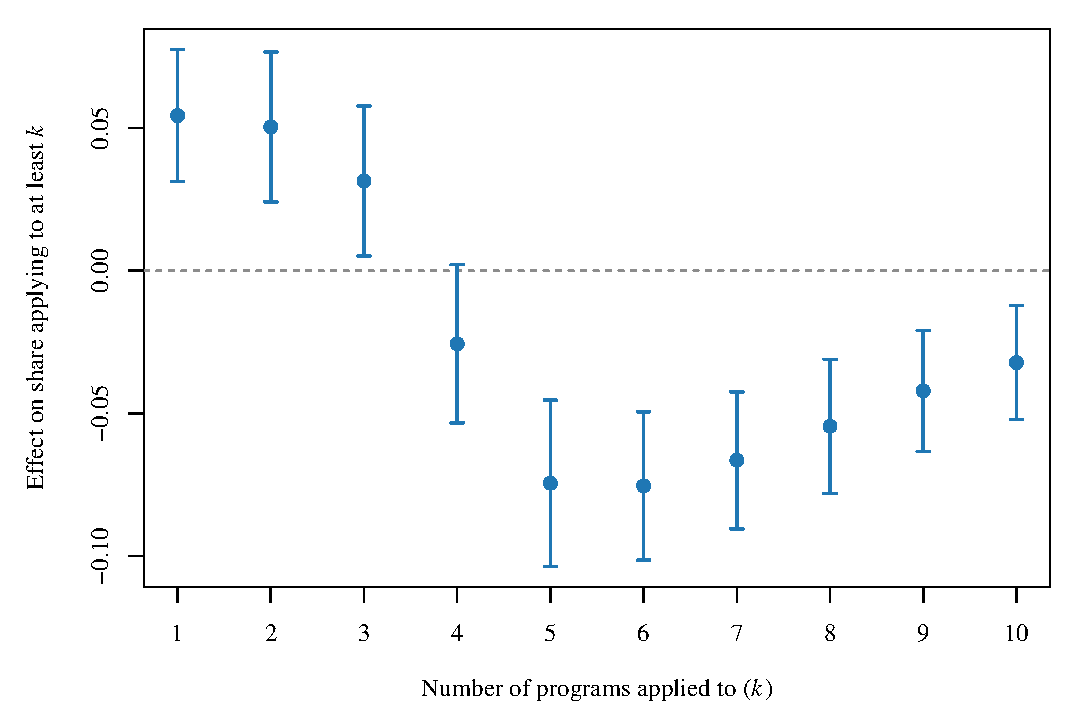
\includegraphics[width=0.8\textwidth]{figures/effect_uniform_errorbars.pdf}
\caption{\marar{Effect of centralized school choice on the share of a class applying to at least $k$ college programs}}
\label{fig: app breadth}
\end{figure}
Furthermore, Table~\ref{tab: effect on truthful reporting} examines whether prior exposure affects preference revelation in the college admissions process. We find a positive and statistically significant effect on truthful reporting of the top-ranked option, indicating that students are more likely to report their most-preferred program first. In contrast, we find no effect on truthful reporting at the bottom of the preference list. 

Taken together, these results indicate that exposure to centralized school choice improves students' understanding of the mechanism and the quality of their college applications, \marar{leading to higher participation and a greater likelihood of admission}.



